%!TEX root = ../report.tex

\begin{document}
    \justifying
    \chapter{Experimental Setup}
    This chapter describes the various selection choices and preparations done to perform the experimentation are presented. We discuss the chosen object detector model, the framework that is used to model and train the model, hyper-parameter tuning, and the selected OOD detection algorithms that are adapted to the object detection task. We also detail various metrics that are used to distinguish between OOD and ID detections.
    
    \section{Object Detection Model}
    In this work we selected \acrshort{ssd} \cite{Liu2016SSDSS} object detection model. The working of \acrshort{ssd} is explained in detail in Section \ref{ssd_background}. We used a pre-trained \acrshort{ssd} model from \acrlong{paz} (\acrshort{paz}) software library introduced by \citet{arriaga2020perception}.
    
    \subsection{\acrlong{paz}}
    \label{paz}
    \acrshort{paz} is a hierarchical library with multiple \acrlong{api} (\acrshort{api}) levels that is proposed to solve various perception problems in robotics domain. It allows for the modification of software pipelines at various hierarchical level based on requirement. Though \acrshort{paz} is similar to previously proposed libraries like TensorFlow Object Detection API (TF-OD) \cite{Huang2017} and Detectron 2 \cite{wu2019detectron2}, the ease of modification to the object detection pipeline in order to incorporate the \acrshort{ood} methods make \acrshort{paz} our library of choice. 
    
    \acrshort{paz} has three levels of abstractions, a high-level abstraction referred to as a Pipeline, consists of application-ready function for object detection, data-augmentation, and input pre-processing, a mid-level abstraction referred to as a Processor. Processors can be used to perform small computations that are needed to provide solutions to various applications or entirely novel algorithms. Hence, introducing flexibility and re-usability of various implemented functions in \acrshort{paz}, a low-level abstraction referred to as a Backend. Backend is meant to be used and modified without any effect on high-level or mid-level functionalities. These backend functions can also be accessed directly without any need for the usage of either Processors or Pipelines. \acrshort{paz} mainly depends on Tensorflow 2.0 \cite{Abadi2016}, OpenCV \cite{opencv} and Numpy \cite{numpy}. In order to ease the implementation and visualizing of the results we also used Matplotlib \cite{Hunter2007}, sci-kit learn \cite{scikit-learn} and seaborn \cite{Waskom2021}.
    
    \subsection{Tensorflow}
    Tensorflow introduced by \citet{Abadi2016} is a library that is initially developed as an internal research tool at Google and later released as open-source software. It is used for the manipulation of tensors that is required in various scientific fields that need intensive numerical calculations. There are multiple \acrshort{api} provided by Tensorflow to make the machine or deep learning models deployable in various devices with \acrshort{cpu}, \acrshort{gpu}, and \acrshort{tpu}. Tensorflow at its current iteration of version $2.\times.\times$ is built using keras \cite{chollet2015keras} as its backend, thereby providing a more hierarchical approach. The integration of keras into Tensorflow enables the implementation and building of neural networks as a graph, or a sequence of configurable modules of neural network layers, loss functions, activation functions along with various regularization and weight-initialization techniques. Tensorflow also provides various special utility functions called Callback functions. These Callback functions are event-triggered and can be used for various tasks like learning rate schedule, early stopping, and logging of various intermediate values.
    
    \subsection{Compute Platform}
    Training any \acrshort{dnn} is a computationally intensive task that involves high-precision multiplication of input images, extracted features, and weights in the order of millions. To optimize the computations, these tasks are run on \acrshort{gpu}. Using \acrshort{gpu} would result in the reduction of training time to hours instead of weeks. In this work, we used the High-Performance Cluster (HPC) available at DFKI, Bremen. The HPC contains a total of 16 compute nodes (12 data storage, 3 GPU-compute, and a login node). Each node consists of two octa-core Xeon E5-2630 v3 (Haswell) aided by a 128GB ECC RAM. Among the three \acrshort{gpu} nodes, two of those nodes are powered by five NVIDIA Titan-XP each with a processing memory of 12GB, and one node has four NVIDIA Tesla V100 cards with 32GB RAM. The resource management and job scheduling are done using Slurm.
    
    \subsection{Training}
    \label{ssd_training}
    In this work, for the training of \acrshort{ssd} object detection model, we used the hyper-parameter setting defined in the original work on \acrshort{ssd} by \citet{Liu2016SSDSS}. These hyper-parameter settings include the number of anchor boxes, size of anchor boxes, batch size, filter sizes of all the \acrshort{nn} layers, loss functions and threshold values for confident scores, \acrshort{iou} overlap scores for non-maximum suppression. We also used the data augmentation techniques that are implemented in the original work. These techniques include random image cropping, random image mirroring, random image expansion, and photometric distortions like modifications in images brightness, contrast, hue, and saturation.
    
    In the original work, the \acrshort{ssd} network is trained using e ”multi-step” learning rate policy in which the learning rate is decreased after a certain number of epochs. The learning rate is decayed using a pre-set decay rate as 0.1, this decay rate is generally referred to as $\textbf{\textit{gamma}}$. To speed up the learning process, we reduced the batch size to a value of 8 and also chose to use Stochastic Gradient Descent (SGD) proposed by \citet{ruder2016overview} with a momentum of 0.9. 
    
    The network is trained for a total of 80 epochs following the above setting and a callback is employed to save all model parameters values to the disk for every 5 epochs. To benchmark the performance of the \acrshort{ssd} object detection network on \acrshort{bdd} dataset, we decided to use the leader board from the object detection competition from the 2018 Workshop of Autonomous Driving. This competition is based on \acrshort{bdd} dataset and the results are not publicly available. But, the runner-ups presented their work titled \textit{CFENet: An Accurate and Efficient Single-Shot Object Detector for Autonomous Driving} \cite{Zhao2018} in which the scores are mentioned. Hence, we decided to use the scores mentioned in their work for bench-marking purposes. According to this work, the winner and runner-up of the competition scored an mAP value of 0.331 and 0.297 respectively.
    
    \section{Out Of Distribution Detection }
    This section describes the implementation of different Out-Of-Distribution (OOD) detection techniques based on the SSD300 object detection model. The methods are originally proposed to solve the task of object classification but are adapted to detect the OOD samples in the area of object detection. 
    
    % \subsection{Max softmax}
    % In this method we extract the softmax scores calculated from the classification head of the SSD300 model are used to classify whether the signal is \acrshort{id} or \acrshort{ood}. We 
    \subsection{ODIN}
    \label{ODIN_methodology}
    In ODIN, the input is perturbed with noise as shown in Equation \ref{perturbation}. To perform ODIN, two forward passes are needed to perturb the input image. In the first pass, a gradient of the loss with respect to the input image is calculated and is scaled using a perturbation magnitude. The input image is modified by subtracting the perturbation calculated in the previous step. This results in an addition of two hyper-parameter Temperature ($T$) and Perturbation magnitude ($\epsilon$). These hyperparameters are tuned using a fraction of test images sampled from \acrshort{idd} dataset. To calculate the gradient we used \textit{tf.GradientTape}, which records all the differentiation operations information, and a sub-method \textit{tf.gradient} calculates the gradient value using the operations that are recorded in the context of the defined tape. 
    
    \begin{figure}
    	\centering
    	\label{fig:pr_basic}
    	\begin{subfigure}[t]{0.485\textwidth}
    		\centering
    		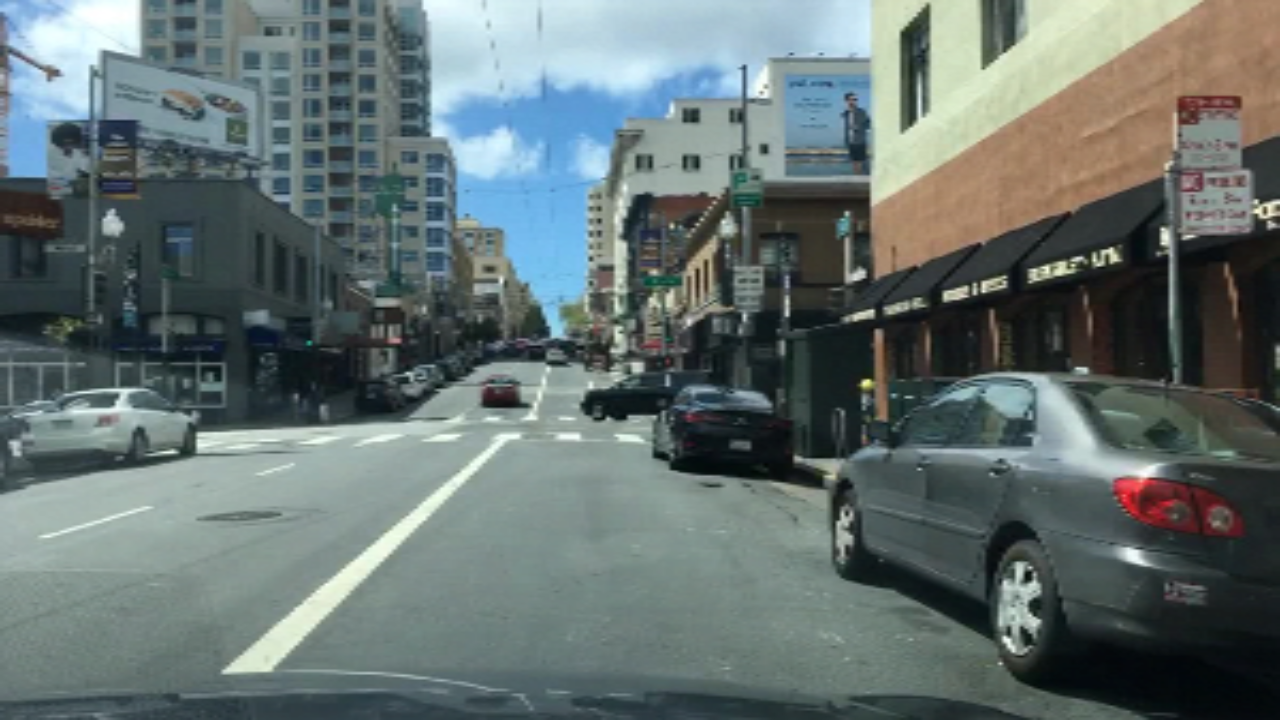
\includegraphics[width=\textwidth]{images/ODIN/image_0.005_10.png}

    		\caption{Perturbation Magnitude=0.005, Temperature=10}
    	\end{subfigure}
    	%
    	\begin{subfigure}[t]{0.485\textwidth}
    		\centering
    		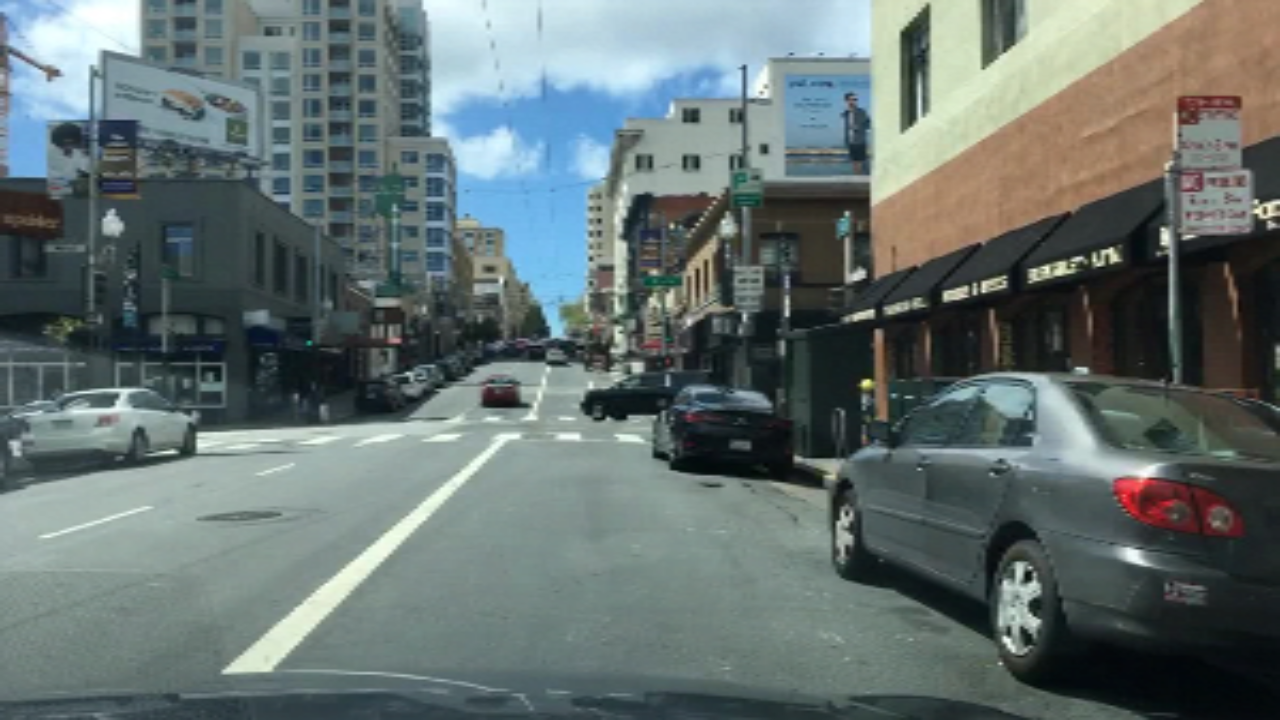
\includegraphics[width=\textwidth]{images/ODIN/image_0.005_1000.png}

    		\caption{Perturbation Magnitude=0.005, Temperature=1000}
    	\end{subfigure}
    % \end{figure}
    
    % \begin{figure} \ContinuedFloat
    	\begin{subfigure}[t]{0.485\textwidth}
    		\centering
    		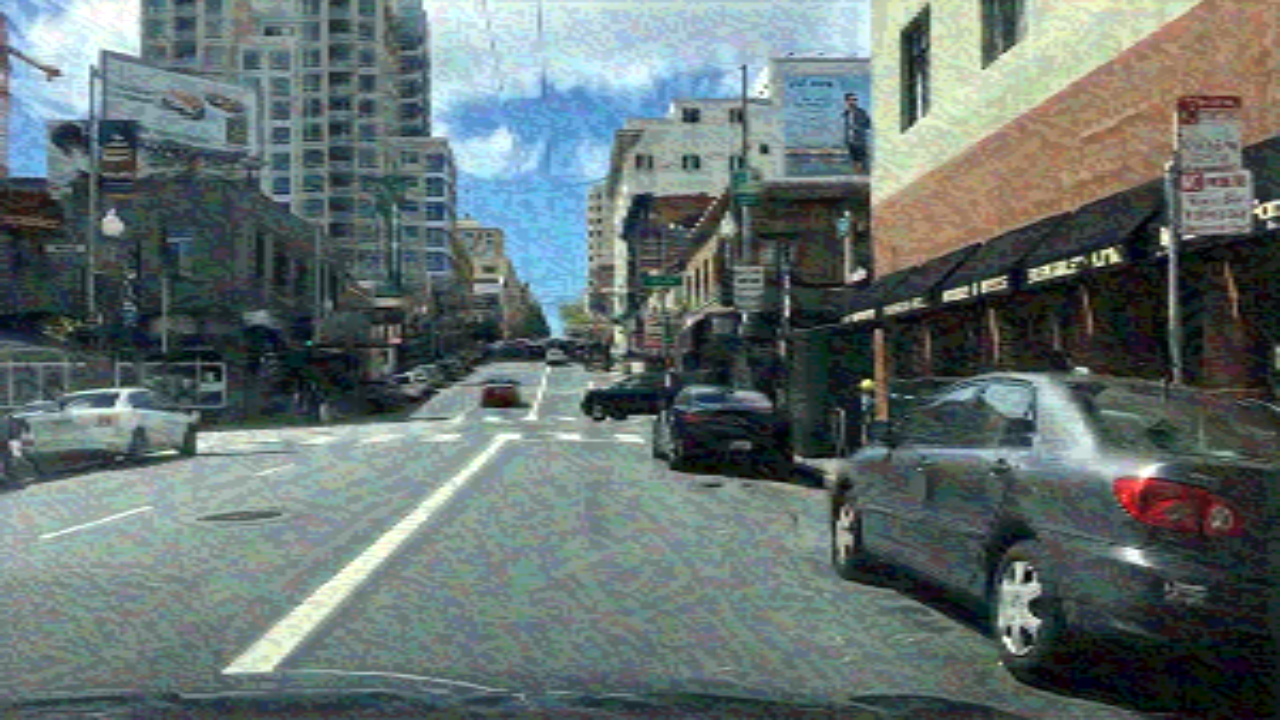
\includegraphics[width=\textwidth]{images/ODIN/image_0.05_10.png}

    		\caption{Perturbation Magnitude=0.05, Temperature=10}
    	\end{subfigure}
        %
    	\begin{subfigure}[t]{0.485\textwidth}
    		\centering
    		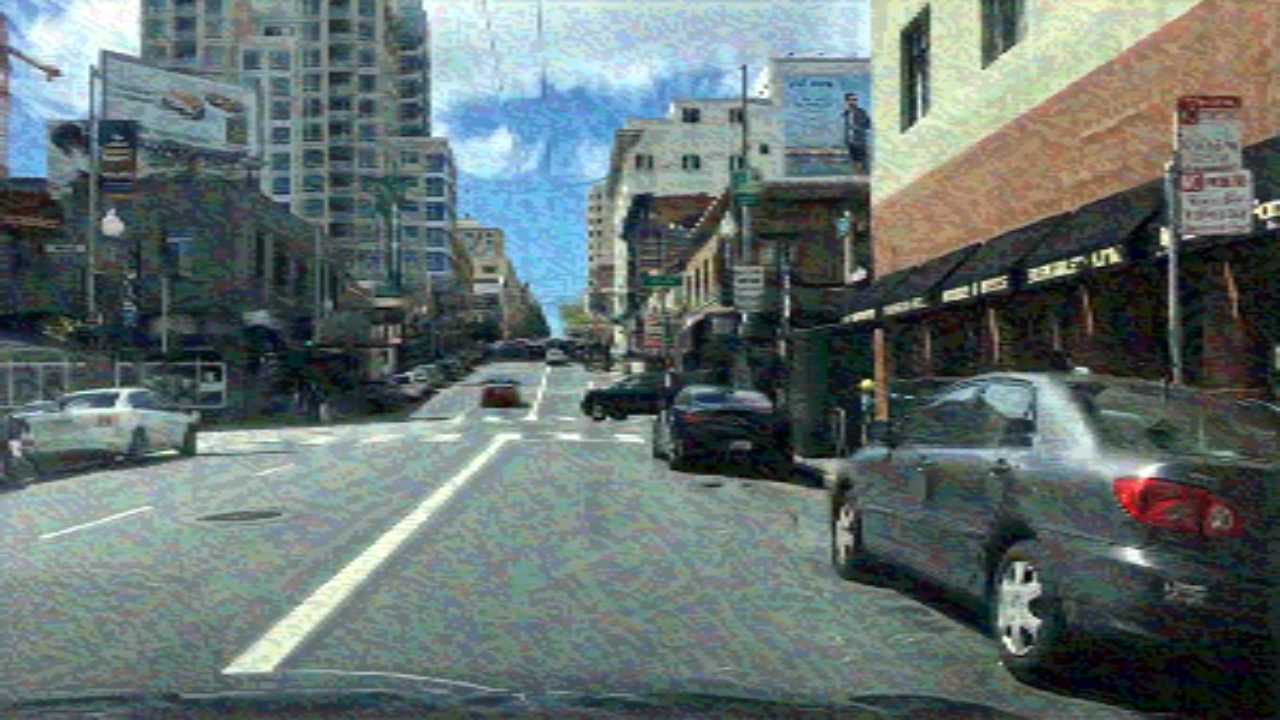
\includegraphics[width=\textwidth]{images/ODIN/image_0.05_1000.png}

    		\caption{Perturbation Magnitude=0.05, Temperature=1000}
    	\end{subfigure}
        
    	\begin{subfigure}[t]{0.485\textwidth}
    		\centering
    		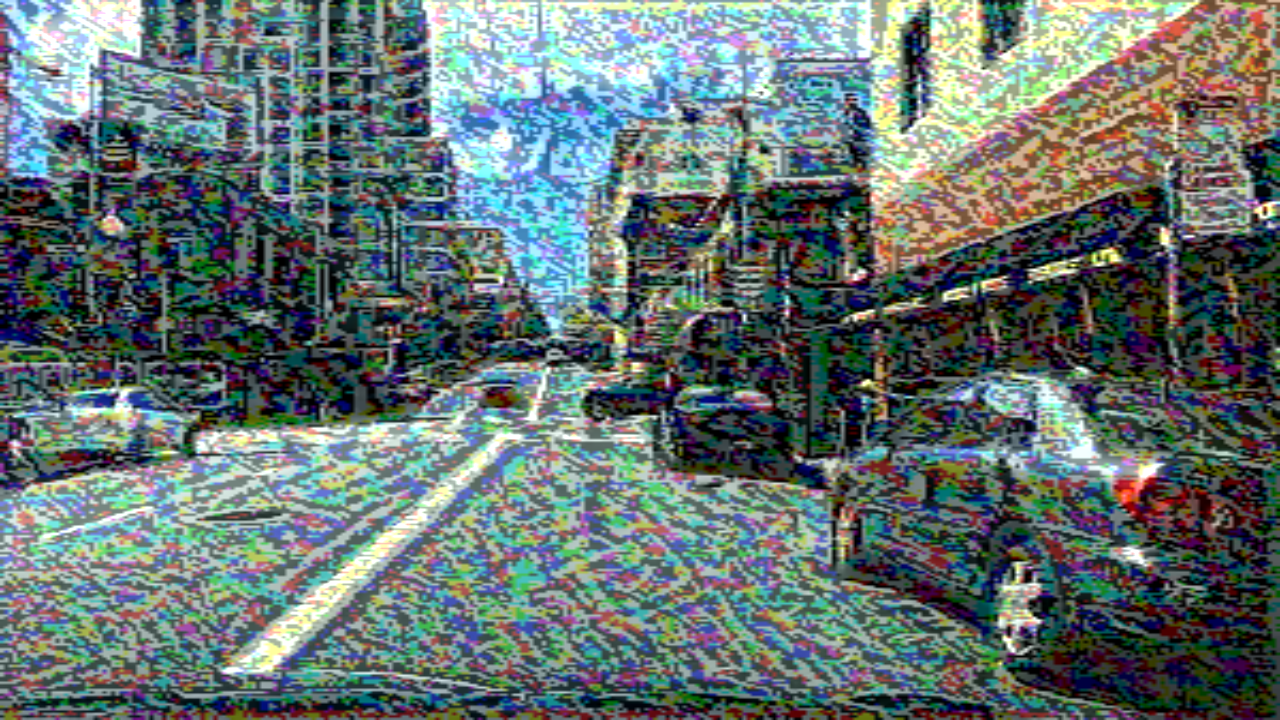
\includegraphics[width=\textwidth]{images/ODIN/image_0.2_10.png}

    		\caption{Perturbation Magnitude=0.2, Temperature=10}
    	\end{subfigure}
        %
    	\begin{subfigure}[t]{0.485\textwidth}
    		\centering
    		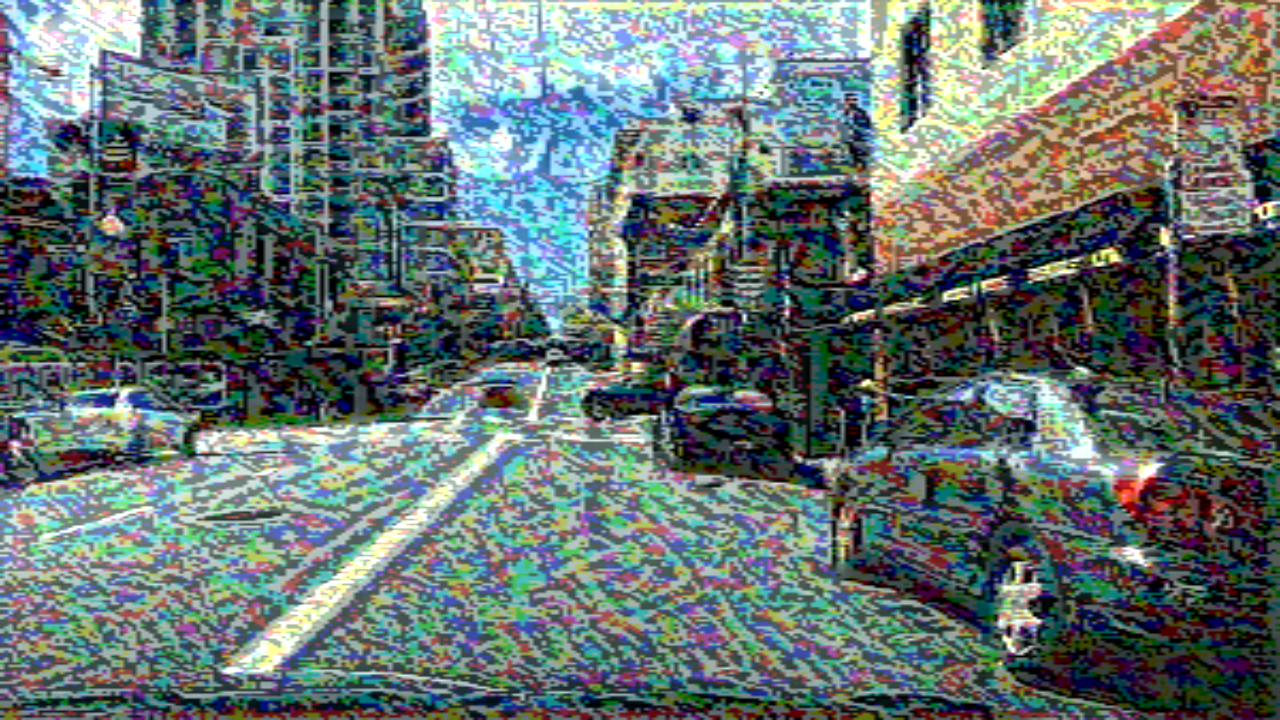
\includegraphics[width=\textwidth]{images/ODIN/image_0.2_1000.png}

    		\caption{Perturbation Magnitude=0.2, Temperature=1000}
    	\end{subfigure}
    
    \caption[Images generated after perturbation and temperature scaling]{Perturbed images with different Perturbation Magnitudes and Temperatures. Observe the increase in the magnitude of noise added to the image with an increase in magnitude and temperature values}
    \label{fig:perturbed_image}
    \end{figure}
    
    \subsection{Mahalanobis Distance based \acrshort{ood} Detector}
    In this method, the training images are used to calculate class-wise mean vectors of each feature and a tied covariance matrix of all the classes using the features from the penultimate layer. The calculation has to be done according to Section \ref{MD_ood}. The class-specific mean vectors and the covariance matrix are used to calculate the Mahalanobis distance of a test sample from each known class. The Mahalanobis distance to the nearest class can be used as a novelty score.
    
    To calculate the mean of class-specific feature vectors and the covariance matrix, we used images with other classes masked out by the mean of the images as shown in Figure \ref{fig:class_specific_image}. This is done to extract exact class-dependent features. 
    
    \begin{figure}
        \centering
        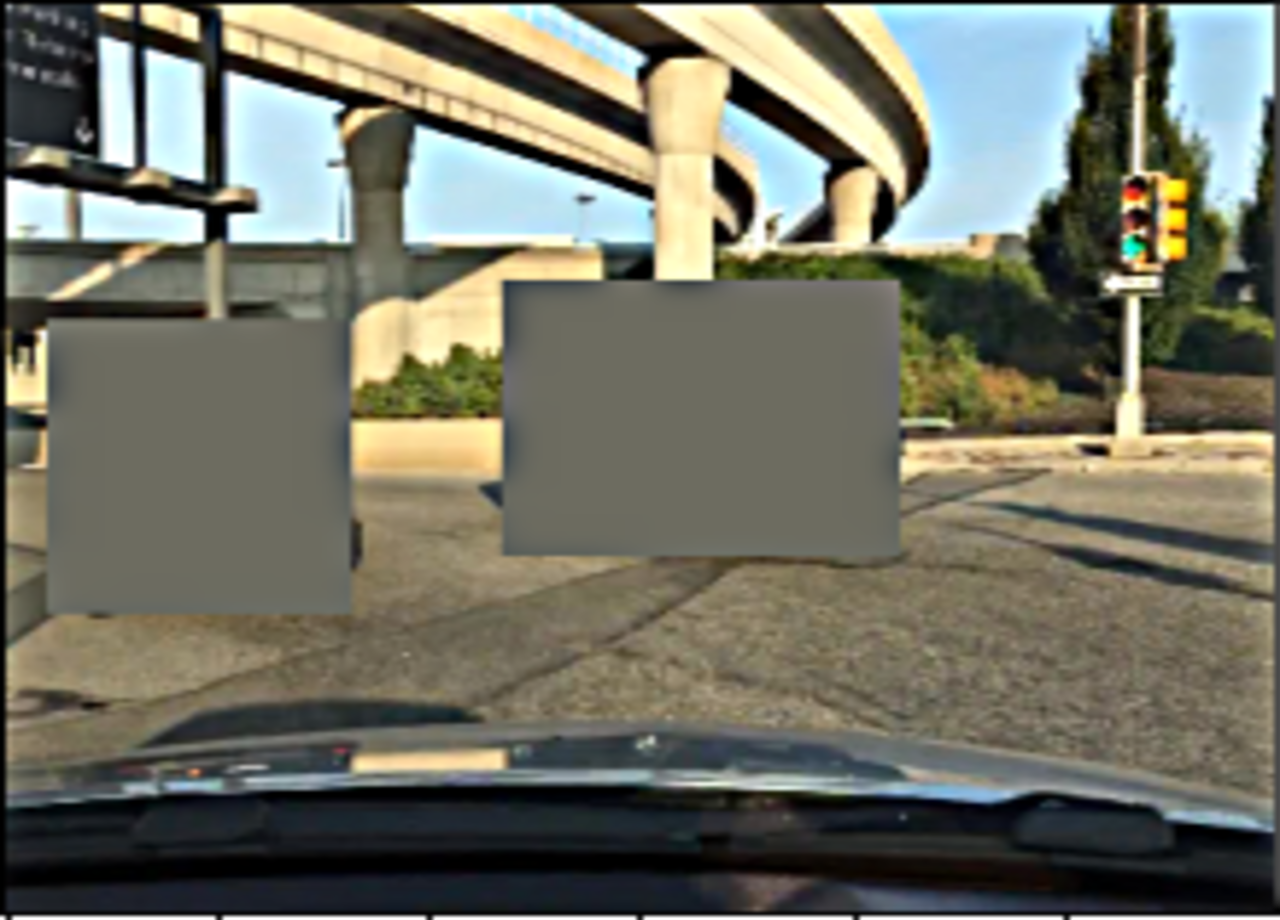
\includegraphics[scale=0.15]{images/MD/rsz_1classspecific-image.png}
        \caption[Class specific images]{Class specific image with all classes masked except Traffic sign}
        \label{fig:class_specific_image}
    \end{figure}
    
    The penultimate layer of the \acrshort{ssd} that is used in this work is \textit{concatenate-2} which is of shape (78588 $\times$ 1). Hence, the covariance matrix is of shape (78588 $\times$ 78588), and calculating it is not possible with the available computational resource present. Hence, we decided not to pursue this as a possible option for an \acrshort{ood} detector in the case of object detection.

    \subsection{Bayesian-SSD Object Detector}
    \label{Bayes-SSD}
    Bayesian-SSD object detector is used to quantify uncertainty in \acrshort{ssd} object detection model. As mentioned in Section \ref{BNN_Intro}, the convolution filters are modeled as a Gaussian distribution parameterized by mean and variance. To model a Bayesian-SSD we used the Tensorflow-Probability library introduced by \citet{Dillon2017}, we use Flipout version of the Convolution layer introduced by  \citet{Wen2018} from the Tensorflow-Probability library to model the Bayesian Layers in the SSD network.
    
    But previous works \cite{Krishnan2020, LaBonte2019} done using the Flipout layers to model the neural network led to the model being under-fitted when trained. We believe the reason for underfitting the model is the inherent stochasticity in weight sampling. To avoid this issue, we decided to only model the layers highlighted in green from the Image \ref{fig:BayesianSSD300}. We adapted the weight initialization proposed by \citet{xavier2010} and initialized the priors with a mean value of \textbf{0} and a standard deviation of \textbf{1}. The Bayesian-SSD300 model is trained similarly to the SSD300 model explained in Section \ref{ssd_training}. 
    
    \begin{figure}
        \centering
        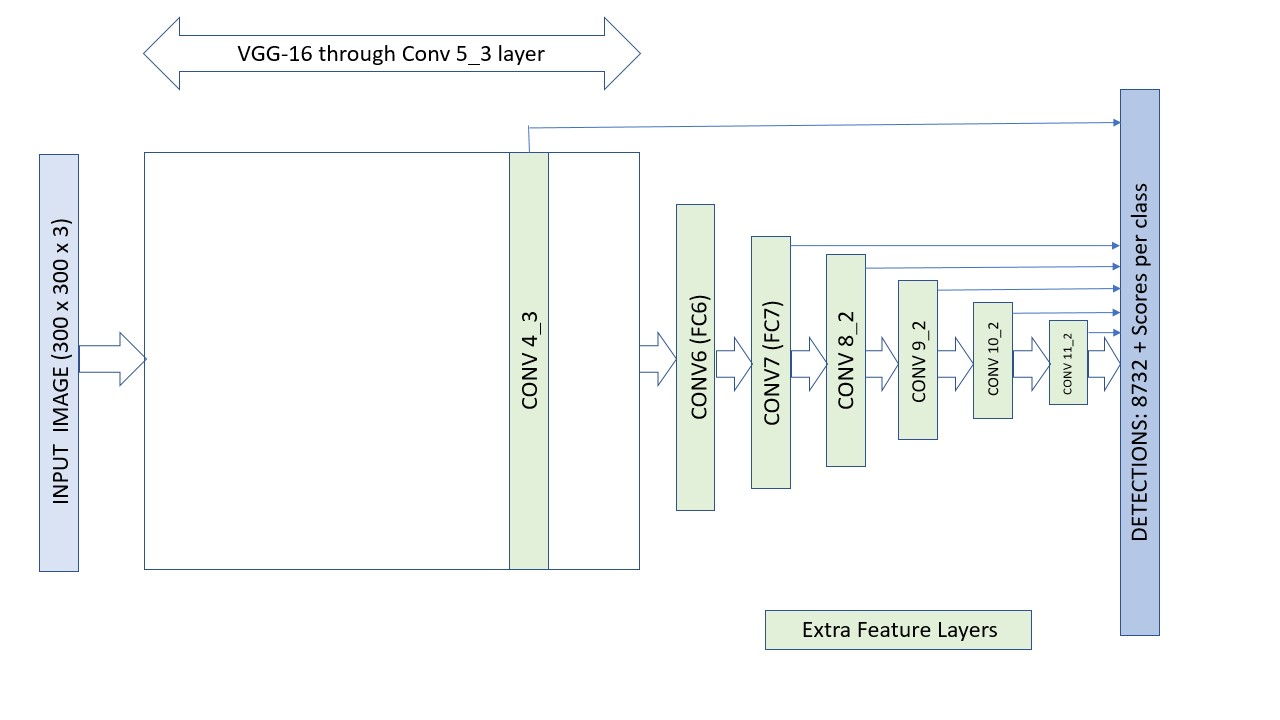
\includegraphics[scale=0.35]{images/frameworks/SSD300_flipout.jpg}
        \caption[SSD object detection model with VGG-19 backbone]{SSD300 model with highlighted layers that are modelled as Bayesian layers}
        \label{fig:BayesianSSD300}
    \end{figure}
    
    To perform uncertainty quantification, we performed \textbf{20} forward passes through the Bayesian-SSD300 model. Since the weights are randomly sampled from the trained prior distributions for every forward pass, each forward pass produces a different output thereby providing an ability to calculate the uncertainty of the SSD300 model in its detections. 
    
    
    \subsection{Sub-Ensemble based SSD Object Detector}
    \label{SSD-subEnsemble}
    In Sub-Ensembles, a model is divided into a trunk network \textbf{T} and a task network \textbf{K}. In this work, we chose the layers highlighted with green color in Image \ref{fig:BayesianSSD300} to be selected as task layers. The rest of the layers in the model are chosen to be trunk network. As already mentioned in Section \ref{deepsubensembles} the trunk network is fixed and will not be trained. Hence, we decided to restore the weights of the trunk network from the best checkpoint of the SSD300 model. 
    
    For training the task network, we initialize all the layers in the task network randomly and are re-trained. Since the initialization of weights is random, training the layers results in a task network having different weights. Hence, every model produces different output for a similar input, this sort of behavior helps us in quantifying the uncertainty in the detections made by the SSD300 model.
    
    To maintain the experiment similarity, we chose to use 20 different task networks to form a sub-ensemble model. Each of the 20 task networks regresses different boxes and the final detection made is the mean of the detections. The different detections made from each task network can be used to produce various uncertainty metrics defined in Section \ref{benchmarking_metrics}.

\end{document}
